\documentclass[10pt,notes,compress,usetitleprogressbar,aspectratio=1610]{beamer}

\usepackage[spanish]{babel}
\usepackage[T1]{fontenc}
\usepackage[utf8]{inputenc}
\usepackage[caption=false,font=footnotesize]{subfig} 		% Separar figuras en subfiguras
\usepackage{multirow}
\usepackage{pdfpages}
\usepackage{graphicx}

\usefonttheme{professionalfonts}
\usepackage{fourier}

\newcommand{\pc}{\ensuremath{\mathit{pc}}\xspace}

\definecolor{palette1}{HTML}{1B9E77}
\definecolor{palette2}{HTML}{D95F02}
\definecolor{palette3}{HTML}{7570B3}
\definecolor{palette4}{HTML}{E7298A}
\definecolor{palette5}{HTML}{66A61E}
\definecolor{palette6}{HTML}{E6AB02}
\definecolor{palette7}{HTML}{A6761D}
\definecolor{palette8}{HTML}{666666}

\usetheme{metropolis}


\usepackage{xspace} % Espaciado correcto detras de comandos.

\usepackage{tikz}
\usepackage{tikztools}
\usetikzlibrary{calc,shapes.multipart,chains,arrows,tikzmark,fit,shapes.geometric}


\newcommand{\nombreautor}{V\'ictor de Juan Sanz\xspace}
\newcommand{\nombretutor}{Desir\'e Garc\'ia L\'azaro\xspace}
\newcommand{\titulo}{Gamificaci\'on: visión general y aplicación en el aula de Matemáticas\xspace}
\newcommand{\TFM}{Trabajo Fin de M\'aster\xspace}
\newcommand{\master}{M\'aster Universitario en Formaci\'on del Profesorado de Educación Secundaria Obligatoria y Bachillerato, Formación Profesional y Enseñanza de Idiomas\xspace}
\newcommand{\especialidad}{Matem\'aticas}

%\newcommand{\nombreautor}{Victor de Juan Sanz\xspace}
%\newcommand{\nombretutor}{Desire Garcia Lazaro\xspace}
%\newcommand{\titulo}{Gamificacion: visión general y aplicación en el aula de Matemáticas\xspace}
%\newcommand{\TFM}{Trabajo Fin de Master\xspace}
%\newcommand{\master}{Master Universitario en Formacion del Profesorado de Educación Secundaria Obligatoria y Bachillerato, Formación Profesional y Enseñanza de Idiomas\xspace}
%\newcommand{\especialidad}{Matematicas}
%\newcommand{\master}{Máster en Formación del Profesorado: especialidad Matemáticas}

\title{\titulo}
\subtitle{\TFM}
\author{Víctor de Juan Sanz}
\date{Julio 2017}
\institute{}

\setbeameroption{hide notes}
%\setbeameroption{show notes}
% \setbeameroption{show only notes}



\begin{document}

\maketitle

\begin{frame}{Índice}
	\setbeamertemplate{section in toc}[sections numbered]
	\tableofcontents[hideallsubsections]
\end{frame}

%%%%%%%%%%%%%%%%%%%%%%%%%%%%%%%%%%%%%%%%%%%%%%%%%%%%%%%%%%%%%%%%%%%%%%
%%%%%%%%%%%%%%%%%%%%%%%%%%%%%%%%%%%%%%%%%%%%%%%%%%%%%%%%%%%%%%%%%%%%%%
%%%%%%%%%%%%%%%%%%%%		Motivación 			%%%%%%%%%%%%%%%%%%%%%%
%%%%%%%%%%%%%%%%%%%%%%%%%%%%%%%%%%%%%%%%%%%%%%%%%%%%%%%%%%%%%%%%%%%%%%
%%%%%%%%%%%%%%%%%%%%%%%%%%%%%%%%%%%%%%%%%%%%%%%%%%%%%%%%%%%%%%%%%%%%%%

\section{La educación de Matemáticas en España}
\note{}

\begin{frame}{Motivación}
	\note{Último 2 de Mayo, se perdió en el espacio por un error de Software.}
	\begin{figure}
		\centering
		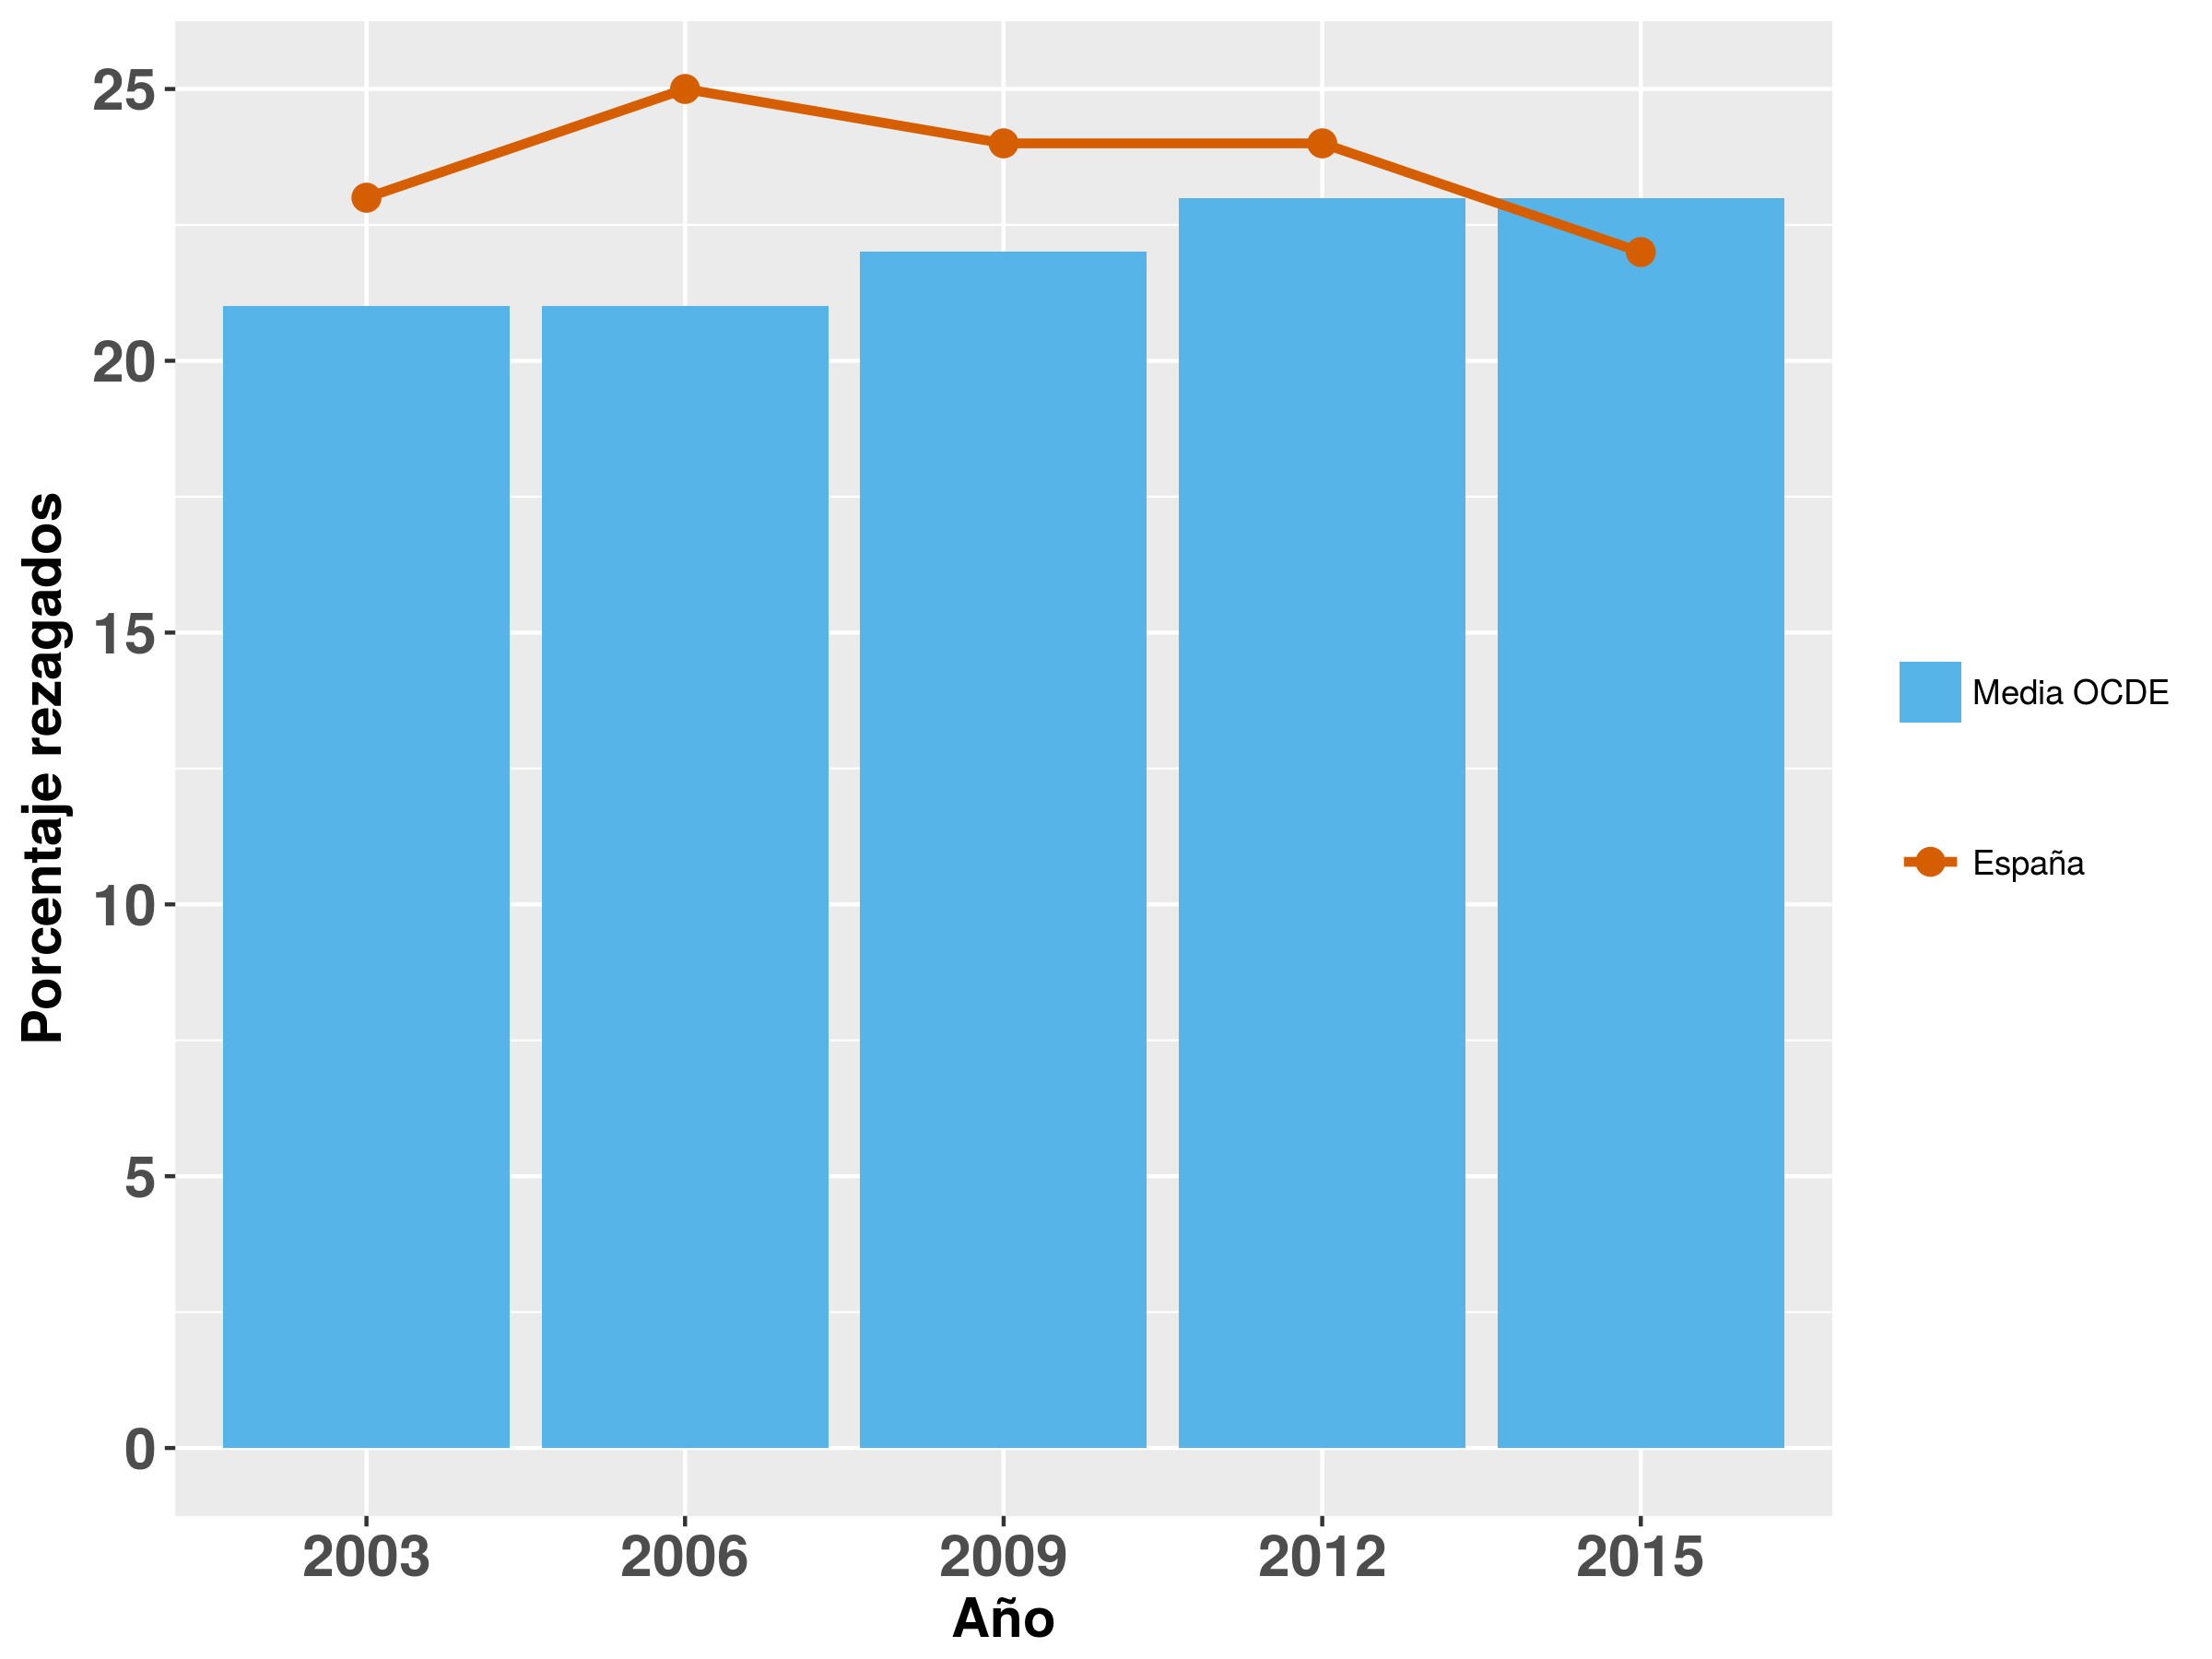
\includegraphics[scale=0.4]{../img/PisaRezagados.png}
		\caption{Estudiantes rezagados en Matemáticas según los informes de Pisa.}
	\end{figure}
\end{frame}

\begin{frame}{Motivación}
	\note{}
	\begin{figure}
		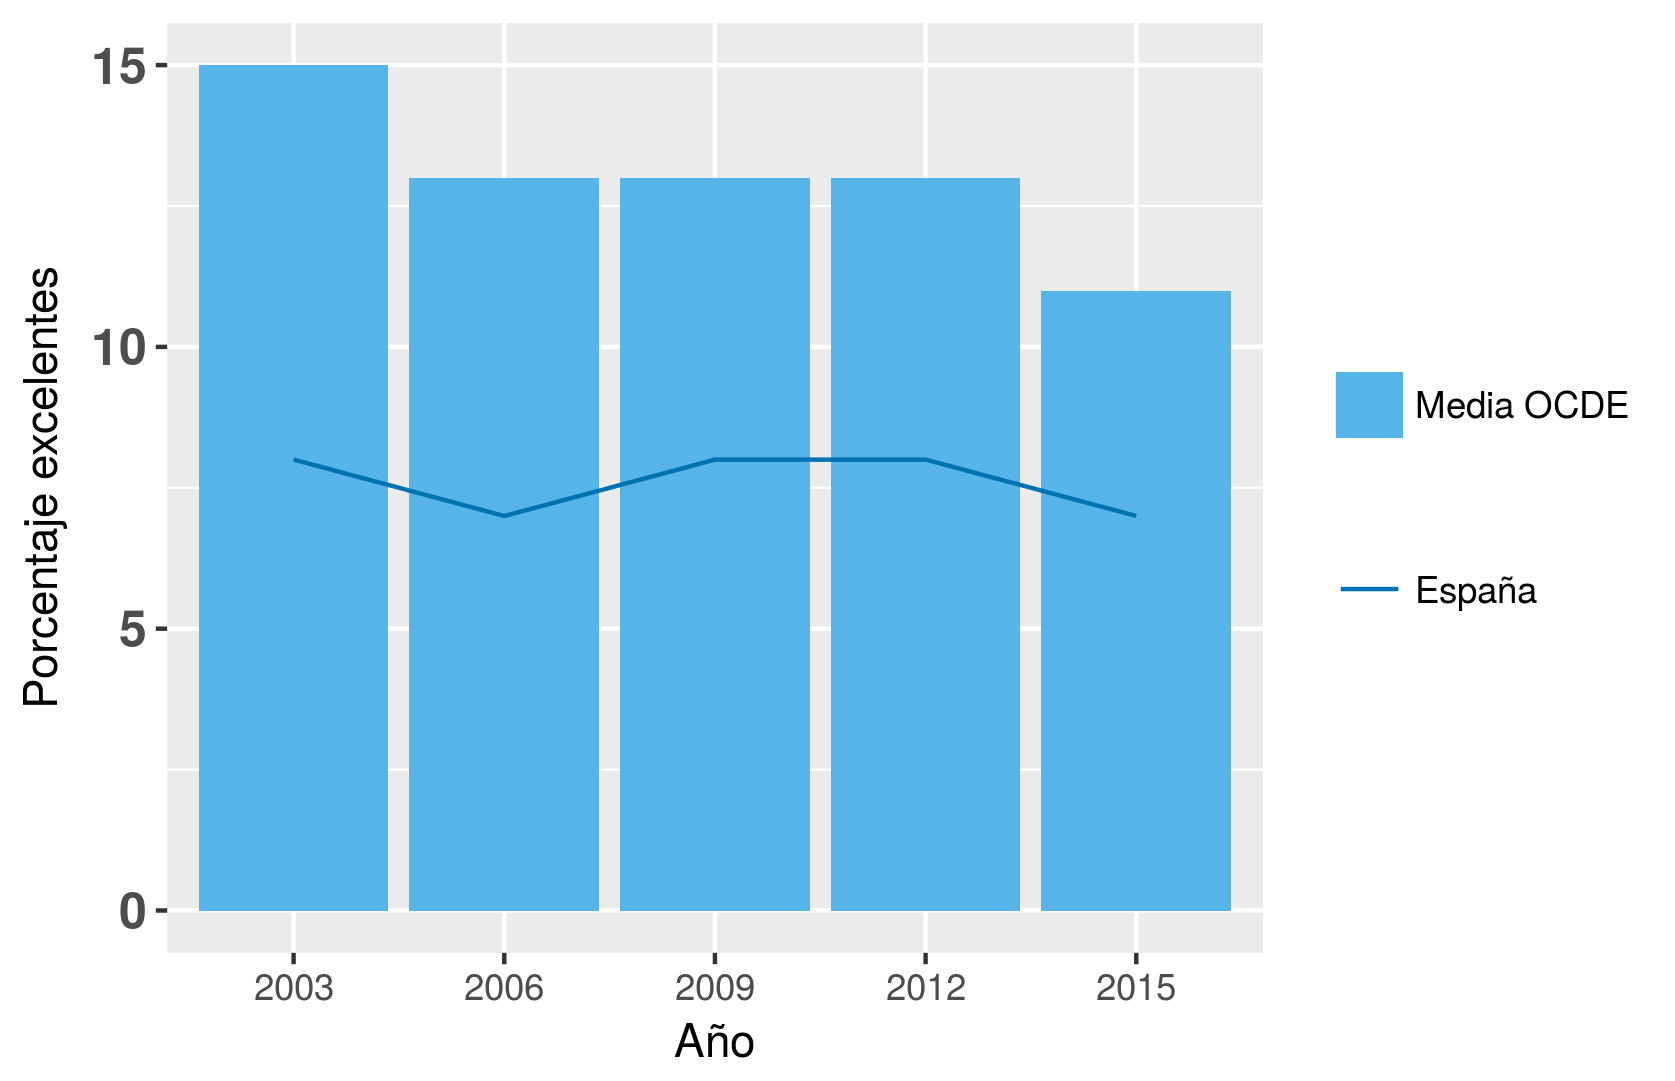
\includegraphics[scale=0.4]{../img/PisaExcelentes.png}
		\caption{Estudiantes rezagados en Matemáticas según los informes de Pisa.}
	\end{figure}
\end{frame}



\begin{frame}{Motivación}
	\note{}
	\begin{figure}
		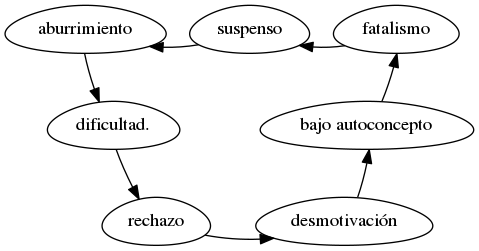
\includegraphics[scale=0.4]{../img/circuloVicioso.png}
		\caption{Circulo vicioso influyente en la actitud de rechazo hacia las Matemáticas según Palacios et al. (2004)}
	\end{figure}
\end{frame}




\section{Objetivos}

\begin{frame}{Objetivos}
\begin{itemize}
	\item Ofrecer una propuesta metodológica para atajar las problemáticas descritas.
\end{itemize}
\end{frame}


\section{La Gamificación como metodología}

\begin{frame}{Definición}
\note{¿Qué más se puede pedir para la enseñanza?}
Kapp (2012) aporta la siguiente definición:
\begin{itemize}
	\item Utilización de mecánicas, estética y procesos de pensamiento de los juegos para involucrar a las personas, motivar su acción, promover el aprendizaje y resolver problemas.
\end{itemize}
\end{frame}


\begin{frame}{Bases teóricas}
\note{
	Algunas teorías en las que se basa la gamificación que han sido estudiadas para la realización del trabajo.
}
Algunas teorías en las que se basa la gamificación:
\begin{center}
\large
	\begin{itemize}
		\item Anatomía de la diversión (Lazzaro, 2004).
		\item Teoría del Flujo (Csikszentmihalyi, 2004).
		\item Teoría de la motivación (E. Deci y Ryan, 1985).
		\item Pirámide de Werbach (Werbach y Hunter, 2012).
		\item Taxonomía de los jugadores (Marczewski, 2015).
	\end{itemize}
\end{center}
\end{frame}

\begin{frame}{Pirámide de Werbach}
	\begin{figure}
		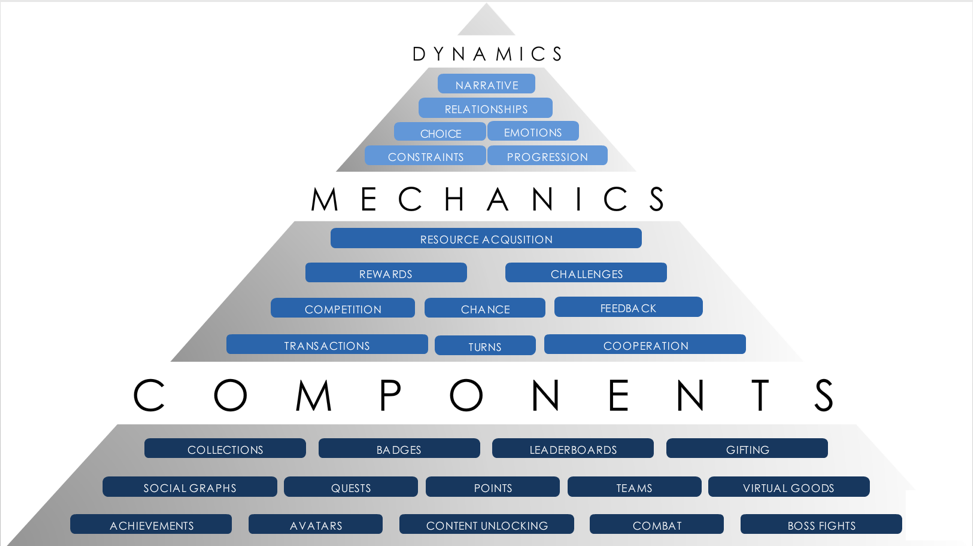
\includegraphics[scale=0.4]{../img/Pyramid.png}
		\caption{Pirámide de los elementos de la gamificación (Werbach y Hunter, 2012)}
	\end{figure}
\end{frame}

\begin{frame}{Taxonomía de los jugadores}
	\begin{figure}
		\begin{center}
			\index{Taxonom\'ia de! Marczewski}
			\label{fig::Marczewski}
			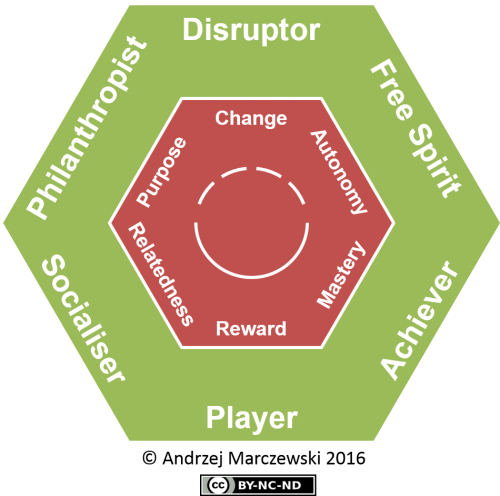
\includegraphics[scale=0.40]{../img/Marczewski.jpg}	
			\caption{Taxonomía de los jugadores según Marczewski.}
		\end{center}
	\end{figure}
\end{frame}


\begin{frame}{Taxonomía de los jugadores}

\begin{figure}[hbtp]
	\begin{center}
		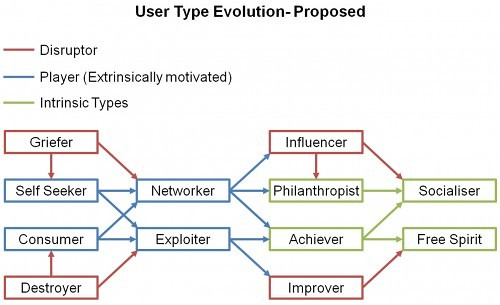
\includegraphics[scale=0.55]{../img/evolution.jpg}
		\caption{Posible conversión de los jugadores según la taxonomía de Marczewski.}
		\end{center}
	\end{figure}
\end{frame}

\subsection{Posibles peligros}
\begin{frame}{Algunos posibles peligros:}
\textbf{Algunos posibles peligros}
\begin{center}
\begin{itemize}
	\item Pointsification.
	\item Explotationware.
	\item Competición.
\end{itemize}
\end{center}
\end{frame}


\section{Propuesta metodológica}
\begin{frame}{Propuesta metodológica}
\note{
	\begin{itemize}
		\item 3 de ESO por el bajón según Palacios et al 2004.
		\item Polinomios por la importancia que tienen.
	\end{itemize}
}
\begin{itemize}
	\item Unidad didáctica en 3 ESO.
	\item Contenido: Polinomios.
	\item Desarrollo de las sesiones: Exposición, trabajo autónomo y trabajo en grupo. Utilización de las TIC (deberes en edmodo).
	\item Materiales: Libro del movimiento Marea Verde.
	\item Deberes en \textit{edmodo}.
\end{itemize}
\end{frame}
 
\newcommand{\eaes}{Estándares de Aprendizaje Evaluables\xspace}

\begin{frame}
	\begin{table}[hbt]
		\centering
		\caption{Matriz de Contenidos, Criterios de Evaluación y  Estándares de Aprendizaje Evaluables de la unidad didáctica}
		\label{tbl:Matrizdetodo}
		\begin{tabular}{|p{0.24\linewidth}|p{0.3\linewidth}|p{0.42\linewidth}|}
		\hline
		 \multicolumn{1}{|c|}{Contenidos} & \multicolumn{1}{|c|}{Criterios de Evaluación} & \multicolumn{1}{c|}{}
		\\\hline

		{Cont. 2.6.1} Transformación de expresiones algebraicas. 
		&
		\multirow{3}{\linewidth}{{C.E. 2.3} Utilizar el lenguaje algebraico para expresar una propiedad o relación dada mediante un enunciado, extrayendo la información relevante y transformándola.\vfill}
		& 
		{E.A.E. 3.1}: Realiza operaciones con polinomios y los utiliza en ejemplos de la vida cotidiana.
		\\\cline{1-1} \cline{3-3} 

		{Cont. 2.6.2} Igualdades notables. 
		&
		& 
		{E.A.E. 3.2}: Conoce y utiliza las identidades notables correspondientes al cuadrado de un binomio y una suma por diferencia, y las aplica en un contexto adecuado. 
		\\\cline{1-1} \cline{3-3} 

		{Cont. 2.6.3} Operaciones elementales con polinomios. 
		&
		&
		{E.A.E. 3.3}: Factoriza polinomios de grado 4 con raíces enteras mediante el uso combinado de la regla de Ruffini, identidades notables y extracción del factor común.
		\\\hline
		\end{tabular}
	\end{table}
\end{frame}


\section{Desarrollo}

\begin{frame}{Desarrollo}

\note{
	\begin{itemize}
		\item Esta es la temporalización de la sesión.
		\item Está todo perfectamente definido y detallado en la memoria.
		\item Algunas sesiones tienen deberes y otras no.
		\item El examen permite comparar esta metodología con otras.
	\end{itemize}
}
\textbf{Temporalización:}
\begin{itemize}
	\item<1-> Introducción a la metodología y repaso con \textit{Kahoot}.
	\item<2-> Introducción a los polinomios mediante un reto de trabajo autónomo.
	\item<3-> Multiplicación de polinomios mediante un reto cooperativo.
	\item<4-> División de polinomios mediante un reto cooperativo.
	\item<5-> Identidades notables. Desafío individual y \textit{recuerdo re\'ampago}.
	\item<6-> Factorización: teoría y métodos básicos.
	\item<7-> Algoritmo de Ruffini.
	\item<8-> Repaso de la Unidad Didáctica en 2 sesiones mediante retos colaborativos.
	\item<9-> Examen (si procede).
\end{itemize}
\end{frame}


\begin{frame}{Desarrollo}
\note{
	Los puntos y logros sirven para la evaluación continua. 
}
\textbf{Elementos de la Gamificación:}
\begin{itemize}
	\item Puntos.
	\item 6 logros. Algunos inesperados, otros con condiciones claras para conseguirlos.
	\item Tienda: pregunta directa en el examen, Botella de Klein impresa en 3D.
	\item Narrativa: historiadores tras al-Karaji, fundador del álgebra.
	\item Elección en los deberes.
\end{itemize}

\end{frame}


\frame[plain]{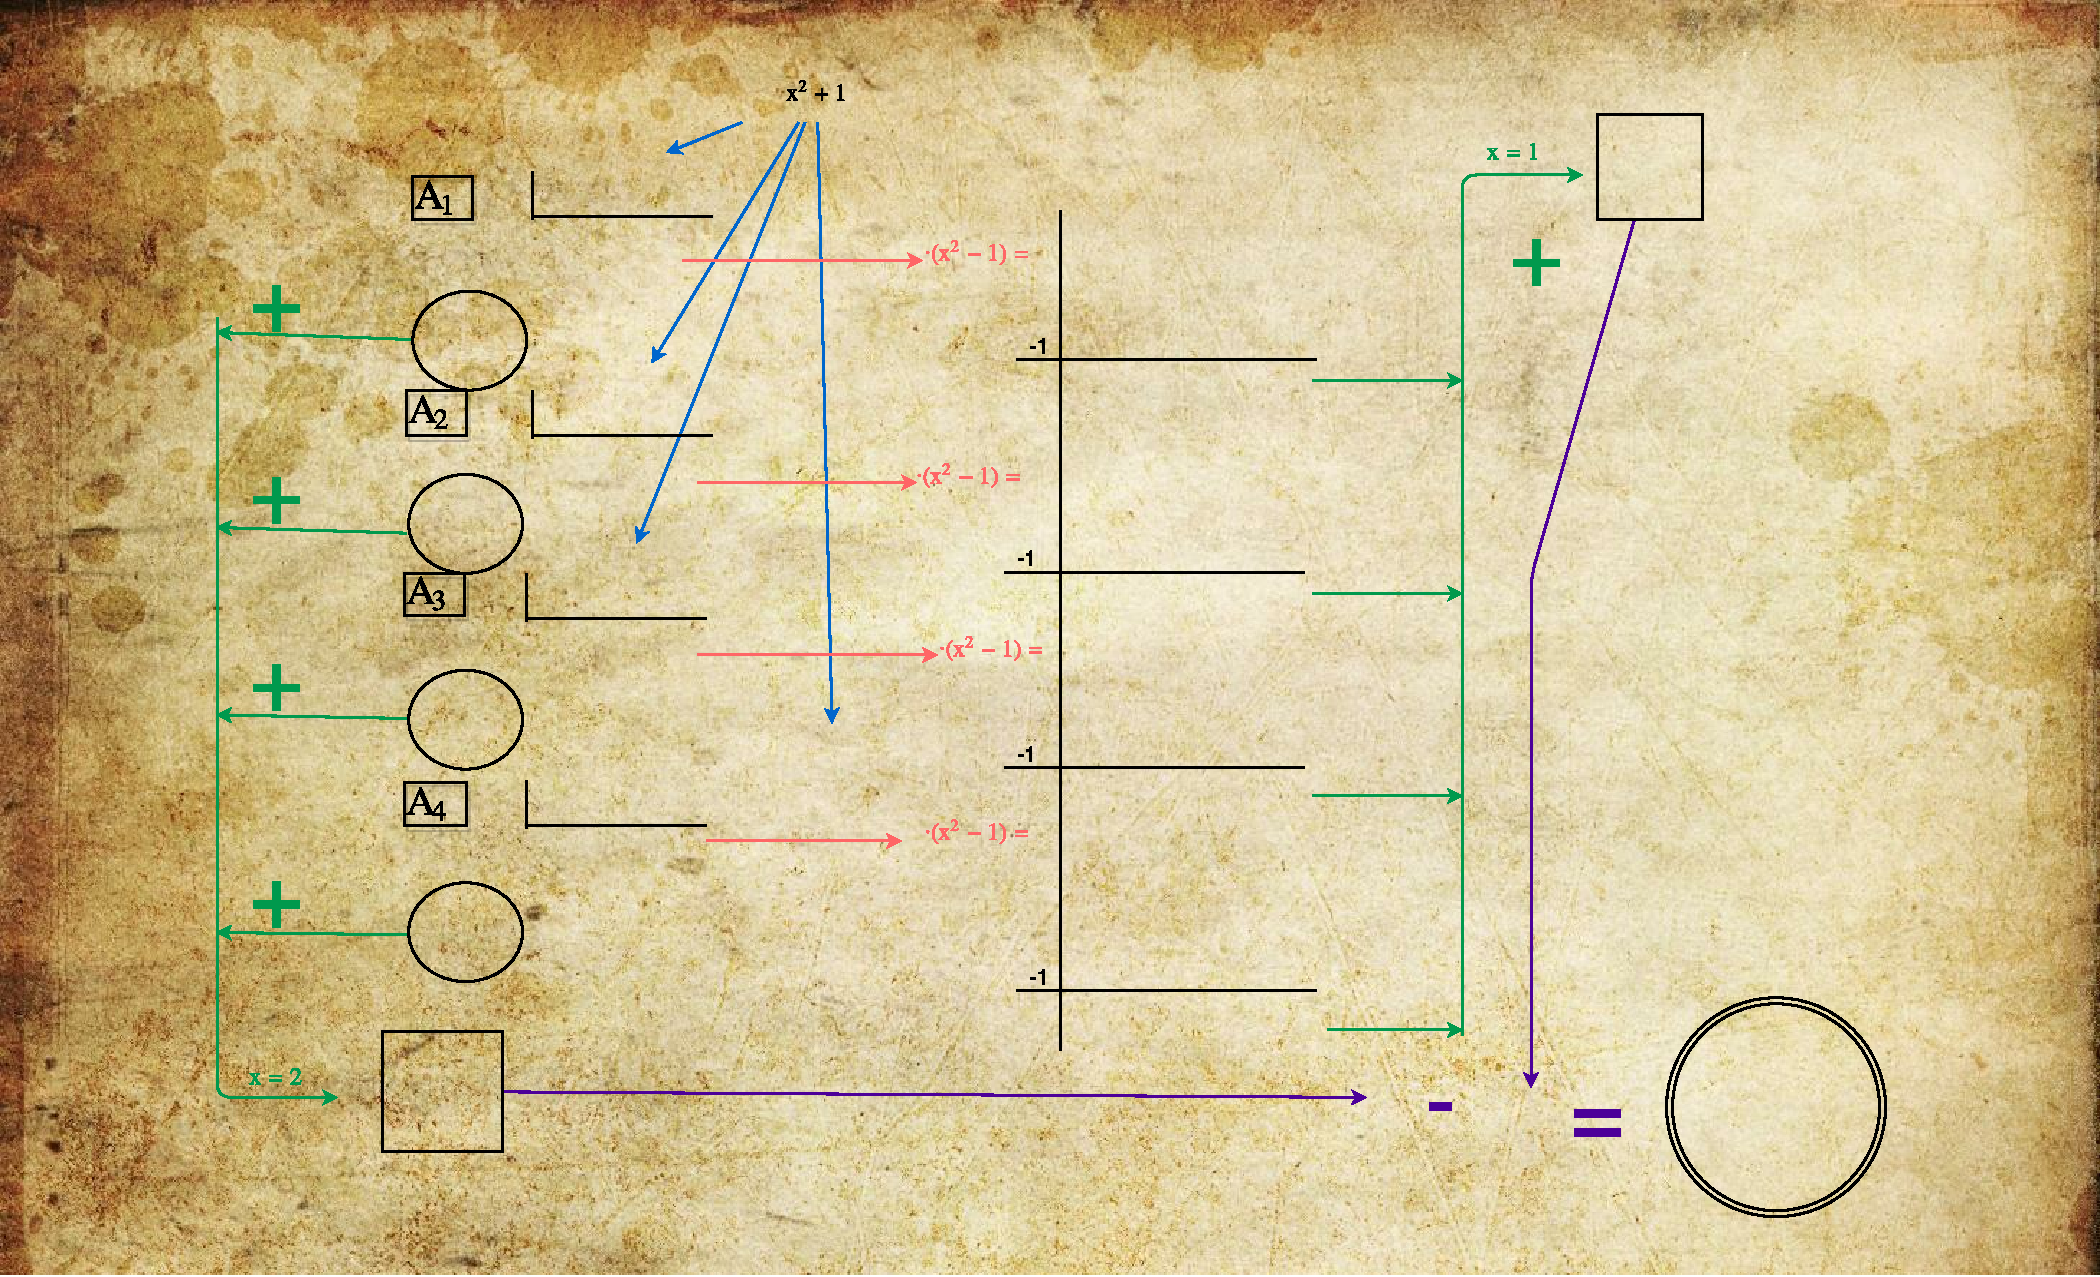
\includegraphics[page=1,width=\textwidth]{../src/RetoCoop.pdf}}





\begin{frame}[standout]
\begin{center}
Muchas gracias por su atención. ¿Alguna pregunta?
\end{center}

\end{frame}

\end{document}
